\documentclass[11pt]{article}

% Package includes

\usepackage{graphicx}
\usepackage{color}
\usepackage{comment}
\usepackage{multirow}
\usepackage{askmaps}
\usepackage{amssymb}
\usepackage{amsmath}
\usepackage{tikz}
\usetikzlibrary{arrows, positioning, shapes.geometric, circuits.logic.US}
\tikzstyle{line}=[draw]
\tikzstyle{arrow}=[draw, -latex]

% Wrap long URLs with hyphens
\PassOptionsToPackage{hyphens}{url}\usepackage{hyperref}
\usepackage{pdftexcmds}
\usepackage{upquote}
\usepackage{textcomp}
\usepackage{minted}
\usepackage[listings]{tcolorbox}
\usepackage{enumerate}
\usepackage{enumitem}
\usepackage{mathtools}
\DeclarePairedDelimiter{\ceil}{\Big\lceil}{\Big\rceil}

\tcbset{
texexp/.style={colframe=black, colback=lightgray!15,
         coltitle=white,
         fonttitle=\small\sffamily\bfseries, fontupper=\small, fontlower=\small},
     example/.style 2 args={texexp,
title={Question \thetcbcounter: #1},label={#2}},
}

\newtcolorbox{texexp}[1]{texexp}
\newtcolorbox[auto counter]{texexptitled}[3][]{%
example={#2}{#3},#1}

\setlength{\topmargin}{-0.5in}
\setlength{\textheight}{9in}
\setlength{\oddsidemargin}{0in}
\setlength{\evensidemargin}{0in}
\setlength{\textwidth}{6.5in}

% Useful macros

\newcommand{\note}[1]{{\bf [ NOTE: #1 ]}}
\newcommand{\fixme}[1]{{\bf [ FIXME: #1 ]}}
\newcommand{\wunits}[2]{\mbox{#1\,#2}}
\newcommand{\um}{\mbox{$\mu$m}}
\newcommand{\xum}[1]{\wunits{#1}{\um}}
\newcommand{\by}[2]{\mbox{#1$\times$#2}}
\newcommand{\byby}[3]{\mbox{#1$\times$#2$\times$#3}}

\newenvironment{tightlist}
{\begin{itemize}
 \setlength{\parsep}{0pt}
 \setlength{\itemsep}{-2pt}}
{\end{itemize}}

\newenvironment{titledtightlist}[1]
{\noindent
 ~~\textbf{#1}
 \begin{itemize}
 \setlength{\parsep}{0pt}
 \setlength{\itemsep}{-2pt}}
{\end{itemize}}

% Change spacing before and after section headers

\makeatletter
\renewcommand{\section}
{\@startsection {section}{1}{0pt}
 {-2ex}
 {1ex}
 {\bfseries\Large}}
\makeatother

\makeatletter
\renewcommand{\subsection}
{\@startsection {subsection}{1}{0pt}
 {-1ex}
 {0.5ex}
 {\bfseries\normalsize}}
\makeatother

% Reduce likelihood of a single line at the top/bottom of page

\clubpenalty=2000
\widowpenalty=2000

% Other commands and parameters

\pagestyle{myheadings}
\setlength{\parindent}{0in}
\setlength{\parskip}{10pt}

% Commands for register format figures.

\newcommand{\instbit}[1]{\mbox{\scriptsize #1}}
\newcommand{\instbitrange}[2]{\instbit{#1} \hfill \instbit{#2}}

\graphicspath{{./figs/}}

%-----------------------------------------------------------------------
% Document
%-----------------------------------------------------------------------

\begin{document}
\def\PYZsq{\textquotesingle}


\newcommand{\headertext}{EE290C CORDIC Lab 2}
\renewcommand{\thesubsection}{\thesection.\alph{subsection}}

\title{\vspace{-0.4in}\Large \bf \headertext \vspace{-0.1in}}
\author{Vighnesh Iyer}

\date{\today}
\maketitle

\markboth{\headertext}{\headertext}
\thispagestyle{empty}

\section{Type Generic CORDIC}
I genericified my CORDIC and found that at least \textbf{27 stages} were required for the \verb|DspReal| version to achieve 2 LSB precision.

I think my usage of typeclasses was excessive, but I just kept adding what was needed to get the code to compile. Is there a way to alias a conjunction of typeclasses like
\begin{minted}{scala}
typeclass CORDICNumber = Data : Ring : BinaryRepresentation : ConvertableTo : Order
\end{minted}

\section{Synthesis}
I modified the \verb|runhammer.sh| script to sweep precision from 8 to 24 in steps of 2 with fixed \verb|stagesPerCycle| of 1 and to sweep \verb|stagesPerCycle| within [1, 2, 4, 8, 16] for fixed precision of 18 (which yields 16 stages). \verb|runhammer.sh| was also modified to run a local Vivado Webpack edition (so I'm synthesizing for a Kintex Ultrascale+ part).

The number of DSPs was always zero, so I'm going to compare the LUT and FDRE utilization versus the module parameters.

I decided to try out \verb|yosys| Xilinx synthesis just for fun.

\begin{figure}[H]
    \centerline{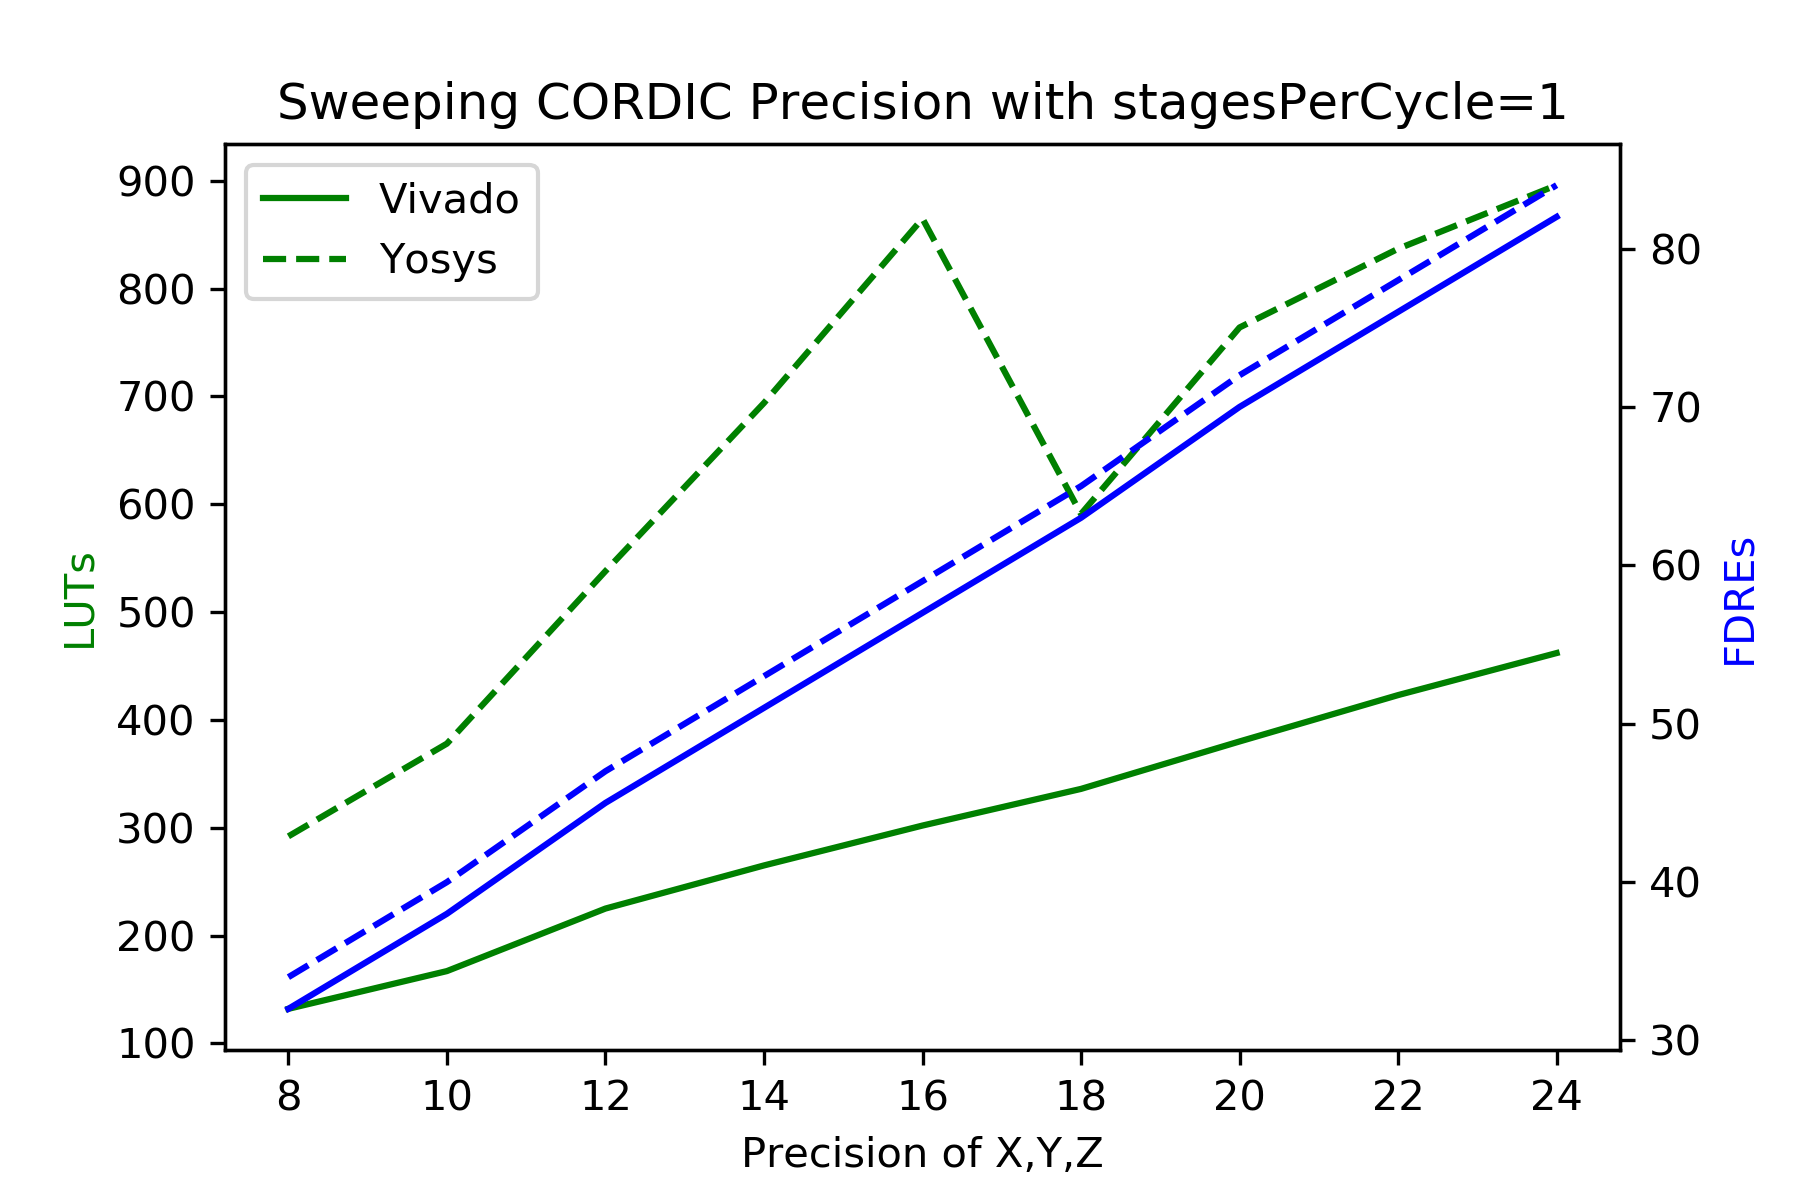
\includegraphics[width=0.7\textwidth]{sweep_precision.png}}
\end{figure}

Yosys appears to be decent at logic optimization (unsurprisingly since it uses Berkeley ABC just as Vivado does for this purpose). But it appears to be a lot worse in LUT packing, at least for this small design. LUT packing is likely something Xilinx has sunk a lot of time into. Yosys uses ABC for LUT packing, but Vivado likely uses something custom.

\begin{figure}[H]
    \centerline{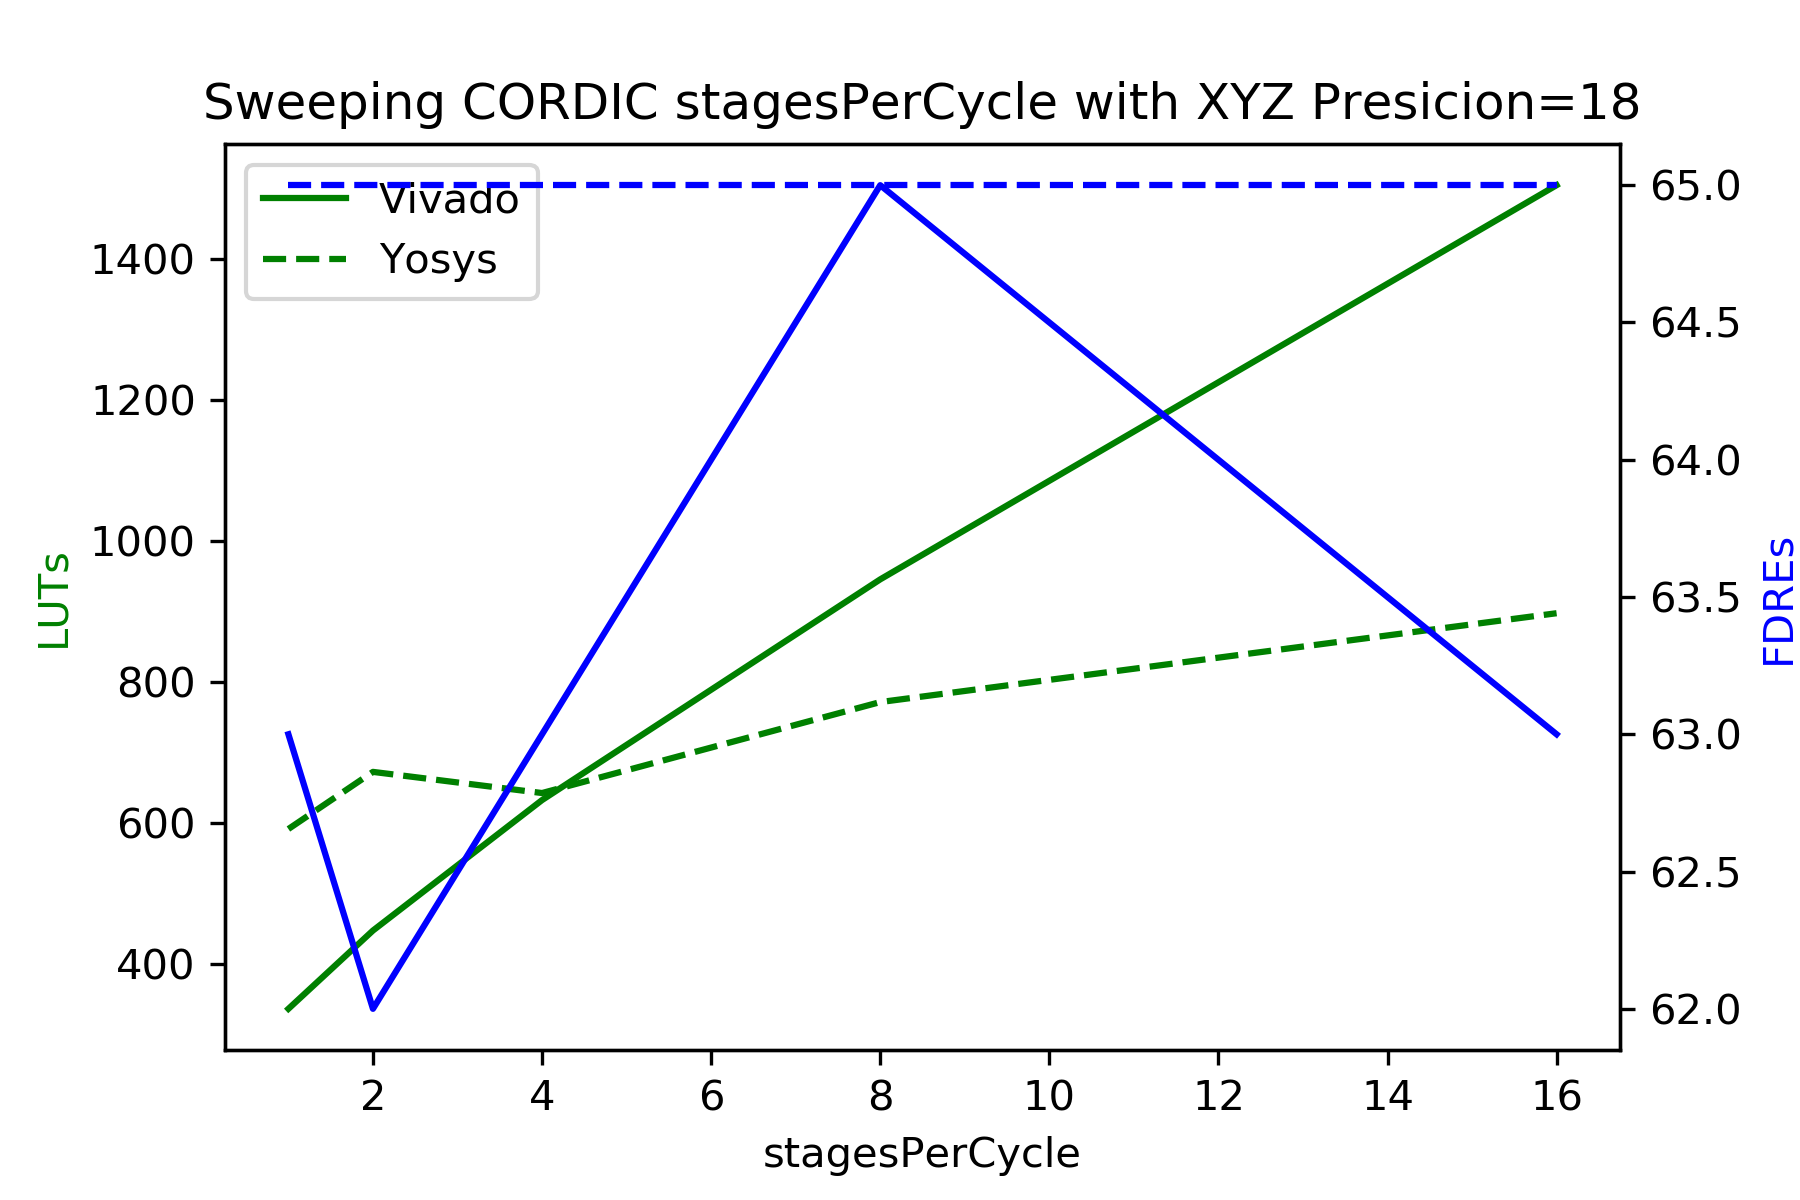
\includegraphics[width=0.7\textwidth]{sweep_stages.png}}
\end{figure}

Here we can see again that Vivado is slighly better at register trimming as it seems to be able to optimize away what I think is the result of my setting the width of my \verb|currentStage| register to \verb|log2Ceil(nStages) + 1|. I think Vivado is able to recode my state machine and extract the savings from this width reduction and knowing that \verb|currentStage| is always incremented by a power of 2 (reducing its number of possible states).

Yosys appears to perform favorably in LUT packing here, probably due to the increased amount of logic being more amenable to ABC's packing algorithm.

\section{Rocket-Chip Integration}
I filled in the template provided to integrate the CORDIC block as a diplomatic TL module. I tested the rotation mode across the same 16 angles I tested in Scala, and dumped the output to \verb|fa18-by/verisim/rotation.out|. A reference output was generated by the \verb|CORDIC.ipynb| notebook and is in \verb|fa18-by/verisim/rotation.gold|. Running \verb|diff --color rotation.out rotation.gold| shows the RTL simulation matches the reference within 0-2 LSBs.

The same files were generated for vectoring mode tests in C (\verb|vectoring.gold| and \verb|vectoring.out|). When it comes to matching $z_{out} = \tan^-1(y)$ all the results are within 1-2 LSBs. But, when looking at the expected value of $x_{out} = \sqrt{x_0^2 + y_0^2}$, the values in the range $y_0 \in [-0.5,0.5]$ all are within 2 LSBs, but the extreme $y_0$ of -1 and 1 give large errors. We never tested this in Chisel simulation, and I think this is caused by overflow with large $y_0$.

\end{document}
